\documentclass[11pt]{article}
\usepackage{dcolumn}
\usepackage[left=1in, top=1in, bottom=1in]{geometry}
\usepackage{graphicx}
\usepackage[table,xcdraw]{xcolor}
\usepackage{longtable}
\usepackage{float}
\usepackage{listings}
\usepackage{xcolor}
\definecolor{commentgreen}{RGB}{2,112,10}

\lstset{language=R,
    basicstyle=\small\ttfamily,
    stringstyle=\color{commentgreen},
    otherkeywords={0,1,2,3,4,5,6,7,8,9},
    morekeywords={TRUE,FALSE},
    deletekeywords={data,frame,length,as,character},
    keywordstyle=\color{blue},
    commentstyle=\color{commentgreen},
}
\begin{document}

\title{Syndicate 5 Statistical Learning Problem Set \#1}
\maketitle
\pagenumbering{gobble}
{\setlength{\parindent}{0cm}



\section*{Credit Card Balances}
\subsection*{Question 1.1}
The expected relationship roughly shows the common sense and logical judgement about the potential relationship between the credit card balance and independent parameters.\\

It is assumed that the credit limit, rating, cards on hand, user’s age and the identity of student could be the main factors that affect the balance of the credit card, which is shown in the following table. Based on these assumptions, detailed regression analysis will be conducted and explained in the following paragraphs. 


\subsection*{Question 1.2}
A multiple linear regression was run with all possible predictors holding ‘balance’ as the outcome and other variables as predictors. Predictors ‘gender’, ‘student’, ‘married’, and ‘ethnicity’ were assumed to be categorical with associated dummy variables created for each predictor.\\ 

Using R, the following coefficients in Table 1 were estimated (see table 8 in appendix).\\
 
Overall, the predictors were effective in explaining the outcome variation. Based on the adjusted R2, 95.36\% of variation in balance was explained by the predictors.\\

As hypothesized, predictors ‘education’, ‘gender’, ‘married’ and ‘ethnicity’ either had a weak or non-significant relationship on credit card balances. Conversely, if the card holder was a student, this was associated with a high balance as previously estimated. Surprisingly, the number of cards held by a customer had a moderate positive association with the balance i.e. the higher number of cards, the higher the balance.

\subsection*{Question 1.3}
Our first model is the same as Q2 except with the $Education$ variable now grouped into three bins based on the likely degree attained. This is to make the regression easier to interpret. The resultant regression is quite good with an Adjusted $R^2$ of 0.954 but we still have many insignificant predictors. However, before removing these, we want to use the second model to avoid any of the common pitfalls of regression.\\

Looking at a correlation matrix of numeric variables, we can see that $Rating$ and $Limit$ are extremely highly correlated and may give us multicollinearity issues. We conducted a Wald test to see if these predictors are jointly useful in predicting $Balance$. 
$$H_0: \beta_{Rating} = \beta_{Limit}$$
$$H_1: \beta_{Rating} \neq \beta_{Limit}$$

The Wald test gives us a p-value of 0.062 which is not enough evidence to suggest that coefficients for $Rating$ and $Limit$ are jointly useful (at the 5\% level). We decided to keep $Rating$ and drop $Limit$ for our second model since it is more likely to dictate the value for each $Limit$ than vice versa, and thus more useful.\\

Before constructing our second model, we first looked at the residuals from Q2 and we see some non-linear patterns in $Income$ and $Rating$ so we chose to include squared terms for our second model. We considered the possibility of interaction terms for this regression however, we couldn't see any likely case the effect of a statistically significant independent variable on the dependent variable would depend on another (statistically significant) independent variable. This model is again quite good with an Adjusted $R^2$ of 0.963, and our new terms being statistically significant (interestingly, with the omission of $Limit$, $Cards$ is no longer statistically significant), but we still have many insignificant coefficients which we can drop to simplify the regression at little cost to accuracy.\\

Thus our third model only has significant terms (all significant at the 1\% level) and maintains the same very high Adjusted $R^2$ of 0.963 with the Residual Std. Error only increasing slightly (88.081 to 88.218). While both model 2 and 3 have similar accuracy, model 3 is preferred due to having fewer terms and thus being easier to interpret. (See table 9 in appendix)\\

\begin{center}
Final Model: $Balance_i = -329.576 - 6.238Income_i -0.021Income_i^2 + 2.471Rating_i + 0.002Rating^2_i - 0.0729Age_i + 428.341Student_i$
\end{center}

% Correlation Table
\begin{table}[!htbp] \centering 
  \caption{Correlation Matrix (numeric data only)} 
  \label{} 
\begin{tabular}{@{\extracolsep{5pt}} ccccccc} 
\\[-1.8ex]\hline 
\hline \\[-1.8ex] 
 & Income & Limit & Rating & Cards & Age & Balance \\ 
\hline \\[-1.8ex] 
Income & $1$ & $0.792$ & $0.791$ & $$-$0.018$ & $0.175$ & $0.464$ \\ 
Limit & $0.792$ & $1$ & $0.997$ & $0.010$ & $0.101$ & $0.862$ \\ 
Rating & $0.791$ & $0.997$ & $1$ & $0.053$ & $0.103$ & $0.864$ \\ 
Cards & $$-$0.018$ & $0.010$ & $0.053$ & $1$ & $0.043$ & $0.086$ \\ 
Age & $0.175$ & $0.101$ & $0.103$ & $0.043$ & $1$ & $0.002$ \\ 
Balance & $0.464$ & $0.862$ & $0.864$ & $0.086$ & $0.002$ & $1$ \\ 
\hline \\[-1.8ex] 
\end{tabular} 
\end{table} 

% Wald Test for Rating and Income
\begin{table}[!htbp] \centering 
  \caption{Wald Test for Rating and Limit} 
  \label{} 
\begin{tabular}{@{\extracolsep{5pt}} cc} 
\\[-1.8ex]\hline 
\hline \\[-1.8ex] 
Wald stat & p-value \\ 
\hline \\[-1.8ex] 
$3.487$ & $0.062$ \\ 
\hline \\[-1.8ex] 
\end{tabular} 
\end{table} 


\subsubsection*{Residual Plots}
\begin{center}
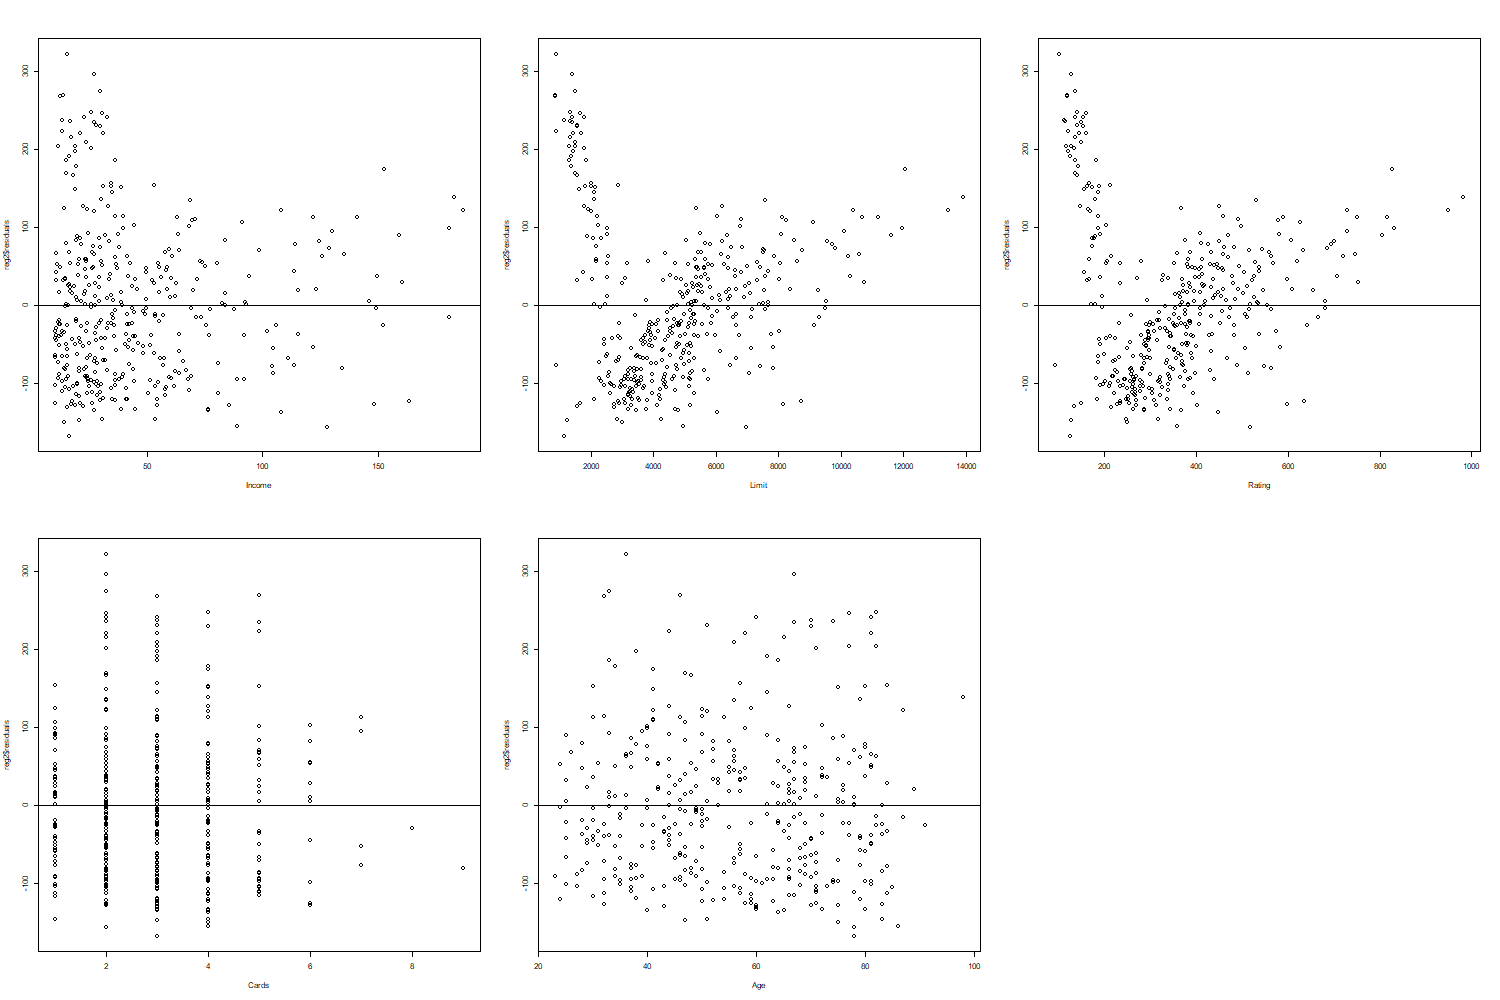
\includegraphics[scale=0.45]{Residual Plots}
\end{center}



\subsection*{Question 1.4}
There are some limitations based on our analysis:\\

In our model, Linear regressions are meant to describe linear relationships between variables. So, if there is a non-linear relationship (student, Ethnicity,), then you will find limitations on it. However, we can sometimes do it by transforming some of the parameters with a log or squared.\\

The basic assumption of linear regression model is the error terms are normally distributed. But there is a possibility that the error terms of the data are at least not perfect normally distributed, or restricted by the limited sample size, the mathematical characteristics of error terms cannot be fully represented. This could lead to the incompleteness and unreliability of the model.\\


\section*{Bank's Marketing Success}
\subsection*{Question 2.1}
$$Pr(y_i = 1|duration_i) = \frac{\exp(\beta_0+\beta_1duration_i)}{1+\exp(\beta_0+\beta_1duration_i)}$$ 
$$Pr(y_i = 0|duration_i) = \frac{1}{1+\exp(\beta_0+\beta_1duration_i)}$$ 


\subsection*{Question 2.2}
$$\ell(\beta|\mathbf{y},\mathbf{X}) = \sum\limits_{i=1}^n \left[ y_i \ln{\left( \frac{\exp(\beta_0+\beta_1duration_i)}{1+\exp(\beta_0+\beta_1duration_i)}\right)} + (1-y_i) \ln{\left( \frac{1}{1+\exp(\beta_0+\beta_1duration_i)}\right)}\right]$$


\subsection*{Question 2.3}
The code used is provided below
% R Output
\begin{lstlisting}[language=R]
## Week 2
## Loading in the data
bank <- read.csv("bankTD.csv", header = TRUE, sep=",")

## Fitting the logistic model using MLE.
## The likelihood function definition.
LL_logistic<-function(beta0,beta1){
  xb=beta0+beta1*bank$duration
  lpy=bank$y*log(exp(xb)/(1+exp(xb)))+(1-bank$y)*log(1/(1+exp(xb)))
  -sum(lpy)
}

## Implementing the MLE
mle_logistic <- mle(minuslogl = LL_logistic, 
                    start = list(beta0=0, beta1=0), method = "BFGS")
summary(mle_logistic)

## Using the glm function
fit1 <- glm(y~duration,binomial(link="logit"),data=bank)
summary(fit1)
\end{lstlisting}

%MLE vs GLM
\begin{table}[H] \centering 
  \caption{mle() vs glm() Output} 
  \label{} 
\begin{tabular}{@{\extracolsep{5pt}}lcc} 
\\[-1.8ex]\hline 
\hline \\[-1.8ex] 
 & \multicolumn{2}{c}{\textit{Dependent variable:}} \\ 
\cline{2-3} 
\\[-1.8ex] & \multicolumn{2}{c}{y} \\ 
\\[-1.8ex] & (mle) & (glm)\\ 
\hline \\[-1.8ex] 
 duration & 0.004 & 0.004$^{***}$ \\ 
  &  & (0.0001) \\ 
  & & \\ 
 Constant & $-$3.180 & $-$3.177$^{***}$ \\ 
  &  & (0.067) \\ 
  & & \\ 
\hline \\[-1.8ex] 
Observations &  & 6,783 \\ 
Log Likelihood & & $-$2,084.980 \\ 
Akaike Inf. Crit. &  & 4,173.960 \\ 
\hline 
\hline \\[-1.8ex] 
\textit{Note:}  & \multicolumn{2}{r}{$^{*}$p$<$0.1; $^{**}$p$<$0.05; $^{***}$p$<$0.01} \\ 
\end{tabular} 
\end{table} 
Note that the mle() function doesn't provide statistical significance, standard errors, observations, a log likelihood or an AIC in its output.


\subsection*{Question 2.4}
\subsubsection*{Nature of Relationship}
The results derived by fitting the logistic model show a positive relationship between the duration of the phone call and the likelihood that a customer takes up the term deposit product offer. Also, the parameters are statistically significant. The model implies the probabilities:\\

If one spends 0 seconds on the phone ($duration_i=0$):
$$Pr(Y=1|duration_i = 0) = \frac{\exp(-3.1768+0.00354 \times 0)}{1+\exp(-3.1768+0.00354 \times 0)} = 0.040$$

If someone spends 1000 seconds on the phone ($duration_i=1000$):
$$Pr(Y=1|duration_i = 1000) = \frac{\exp(-3.1768+0.00354 \times 1000)}{1+\exp(-3.1768+0.00354 \times 1000)} = 0.197$$

\subsubsection*{Odds Ratio}
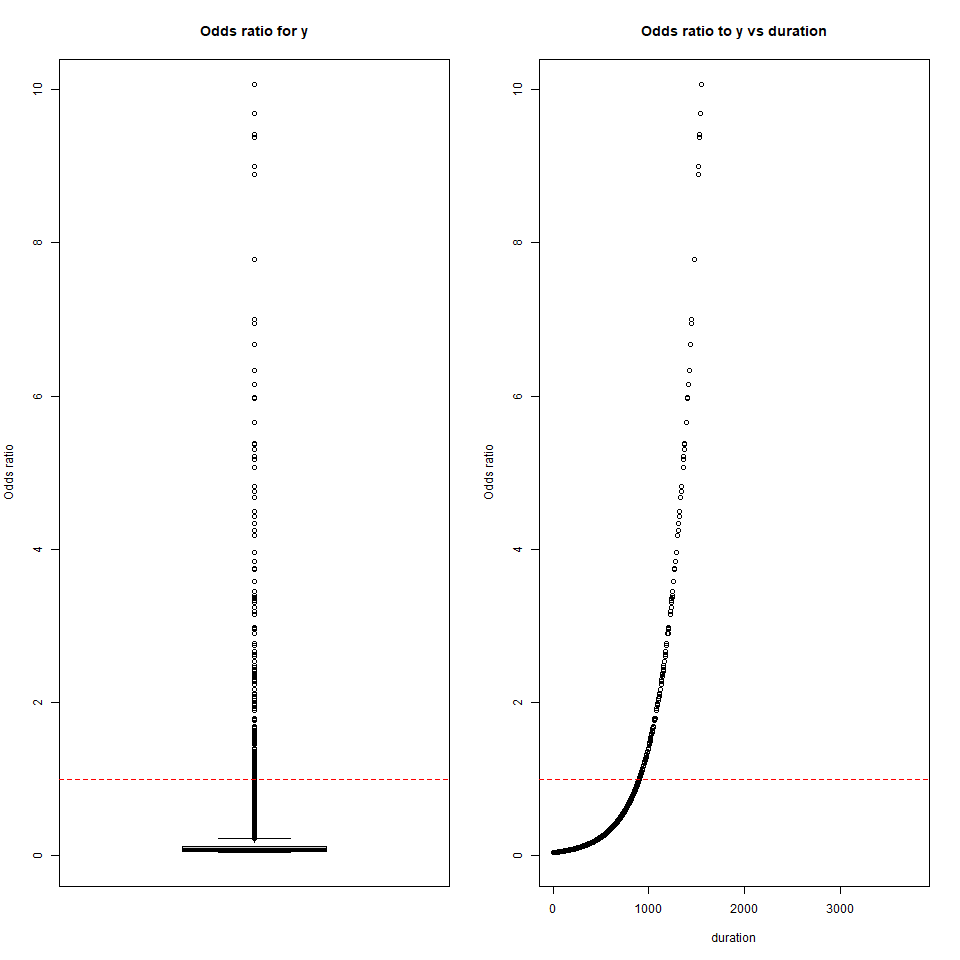
\includegraphics[scale=0.35]{Odds}\\

Since $\beta_1$ is positive (0.00354), the odds ratio is going to increase with the duration. The below figure shows a similar tendency as predicted. Initially, we conduct odds ratio among all data, the extreme values make a vague result. Thus, we limit the range of odds ratio to (0,10) to have a clear result. The red line (Odds ratio = 1.0) is a reference indicating that the probability of subscribing to a term deposit is equal to the probability of not subscribing. Individuals with longer duration calls (more than about 900 seconds) are more likely to sign up for the term deposit.  

$$Pr(Y=1|duration_i = 900) = \frac{\exp(-3.1768+0.00354 \times 900)}{1+\exp(-3.1768+0.00354 \times 900)} = 0.502$$
$$Pr(Y=0|duration_i = 900) = \frac{1}{1+\exp(-3.1768+0.00354 \times 900)} = 0.498$$
$$Odds_i = \frac{Pr(y_i=1|X_i)}{Pr(y_i=0|X_i)} = \frac{0.502}{0.498} = 1.008$$

\subsubsection*{Marginal Effect}
Also, positive $\beta_1$ implies that an increase in the duration of the call has positive impact on the propensity. The marginal effect can be calculated from:

$$ME_i = \frac{\beta_1 \exp(X_i \beta)}{(1+\exp(X_i \beta))^2}$$

In this part, we choose a couple of data points to illustrate the marginal effects.\\

If customers spend 255 seconds (mean) on phone call:
$$ME_i = \frac{0.00354 \exp(-3.1768 + 0.00354 \times 255)}{(1+\exp(-3.1768 + 0.00354 \times 255))^2} = 0.0003$$

If customers spend 900 seconds (mean) on phone call:
$$ME_i = \frac{0.00354 \exp(-3.1768 + 0.00354 \times 900)}{(1+\exp(-3.1768 + 0.00354 \times 900))^2} = 0.0009$$

As calculated, with the increase of duration, the magnitude is larger indicating that customers’ propensity to take up the term deposit is increasing. 

\subsection*{Question 2.5}
Building on the model created in Section 2.3, other variables including job type, marital status, education, credit default, balance, housing, personal loan, previous contact and previous outcome information were included in the model as predictors. Using R, the following coefficients and p-values were estimated. (See table 10 in appendix)\\

Based on these results, age, marital and credit default were not significant in the model. Conversely, call duration and whether the customer signed up to the previous marketing campaign had a significant and positive effect on whether the customer signed up to the term deposit. Additional predictors, such as, whether the customer had a housing or personal loan with the bank had a significant negative effect i.e. if the customer had another home or personal loan with the bank, they were less likely to open a further term deposit.\\

Predictors within the job and education categories had mixed results. Customers with tertiary education were significantly more likely to sign up to the term deposit compared to customers with only primary education (reference group). However, customers with secondary or unknown education were not significantly different from those with primary education only. Within the jobs category, customers that were within blue collar, technician, entrepreneur and management type roles were significantly less likely than those in admin jobs (reference group) to sign up for the term deposit. In contrast, students were significantly morel likely to open a term deposit than customers in admin jobs. All other jobs were not deemed significantly different from admin roles.\\

\subsubsection*{Single and Multiple Predictor Model Comparison}
To understand if the multiple predictor model improved upon the single predictor model from Section 2.3, the AIC values were compared. The table below summarises the deviance and AIC values for the null, single parameter and multiple parameter models. The AIC value was significantly reduced in the multiple predictor model compared to the single predictor model. This indicates that the multiple predictor model is a better predictor of whether customer will sign up for the term deposit than the single predictor model, hence is an improvement upon the single predictor model. Both multiple and single predictor models perform better than the null model based on the AIC.\\

\begin{table}[!htbp] \centering 
  \caption{Deviance and AIC Comparison} 
  \label{} 
\begin{tabular}{@{\extracolsep{5pt}} cccc} 
\\[-1.8ex]\hline 
\hline \\[-1.8ex] 
 & Null & Single Predictor & Multiple Predictors \\ 
\hline \\[-1.8ex] 
Deviance & $4,897.606$ & $4,169.960$ & $3,460.514$ \\ 
AIC & $4,899.606$ & $4,173.960$ & $3,514.514$ \\ 
\hline \\[-1.8ex] 
\end{tabular} 
\end{table} 

To further evaluate if the single and multiple predictor models were significantly different, a likelihood ratio test was completed. The null hypothesis was that all coefficients of the added predictors would equal zero, with the alternative hypothesis being that these coefficients would not equal zero. Results from the likelihood ratio test were as follows:\\

\begin{itemize}
\item Likelihood Ratio (LR) = 709.45 
\item p-value = 0 
\end{itemize}

The p-value from the likelihood ratio test indicates that the multiple predictor model is significantly different from the single predictor model. Hence the multiple predictor model is a statistically significant improvement on the single predictor model.  

\subsection*{Question 2.6}
The logistic regression model with multiple regressors originates from Section 2.5. In this section, this model is revised further by adjusting the reference groups, incorporating non-linear terms, and removing insignificant terms. The model selection process follows a large-to-small method and evaluates the statistical significance (p-value) of individual predictors and the overall AIC value of each model iteration. The model selection process is summarised below:\\

Step 1: Changing reference groups of categorical regressors:\\
\begin{itemize}
\item From the previous model, the estimate coefficient of job group “unemployed” was found to be statistically insignificant (p-value = 0.394). Hence, the reference group of job was changed from “admin” to “unemployed” in the regression. Intuitively, it was also easier to interpret customers with different job types against unemployed customers. 
\end{itemize}
Step 2: Adding the nonlinear terms:\\
\begin{itemize}
\item Quadratic terms for balance and call duration were added to the model to account for the variable effects at larger values. Intuitive, customers with extremely high balance would be more inclined to open a term deposit. Similarly for call duration, if the customer showed great interest in the campaign (by staying on the call for a longer duration), the customer would be more likely to sign up the term deposit.
\item Interaction terms were also added based on intuition. Customers with home and personal loans were likely previously contacted by the bank to setup the loan. Hence, there was a likely interaction between customers with home and personal loans with the bank and customers with a higher number of previous contacts.
\end{itemize}
Step 3: Dropping insignificant terms:  
\begin{itemize}
\item The significant level was set at 20\%. Hence, after each iteration, only significant terms were retained in the model. In the final model, age, previous outcome, and the interaction term of previous and loan were deleted from the model. 
\end{itemize}
The Selection process is conducted as (see table 11 in appendix):\\

\begin{table}[!htbp] \centering 
  \caption{} 
  \label{} 
\begin{tabular}{@{\extracolsep{5pt}} ccccc} 
\\[-1.8ex]\hline 
\hline \\[-1.8ex] 
 & Null & Model (1) & Model (2) & Model (3) \\ 
\hline \\[-1.8ex] 
Deviance & $4,897.606$ & $3,460.514$ & $3,305.273$ & $3,311.087$ \\ 
AIC & $4,899.606$ & $3,514.514$ & $3,367.273$ & $3,363.087$ \\ 
\hline \\[-1.8ex] 
\end{tabular} 
\end{table} 



\subsubsection*{Likelihood Ratio Test}
A further Likelihood Ratio test was run to compare if the initial  Model (1) was significantly different from the final model Model (3). The null hypothesis was defined by assuming that the coefficients of the removed predictors from Model (1) to Model (3) were equal to zero i.e. there was no difference between Model (1) and Model (3). The alternative hypothesis was that the coefficients of the removed predictors were not equal to zero. The results were as follows:\\
\begin{itemize}
\item Likelihood Ratio (LR) = 149.42
\item p-value = 0
\end{itemize}

Based on the p-value, the likelihood ratio test indicates that the final model, 
Model (3) is significantly different from the initial model, Model (1).  

\subsection*{Question 2.7}
The cut-off point in the logistic regression model represents the border of predicted true or false predictions. Given the regression model explained before with 50\% cut-off rate, the precision of the model is 64.1\%, the error rate with false negative is 8.07\%, and the error rate of false positive is 35.9\%, as shown in the following table.\\

%Hit and Miss Table
\begin{table}[!htbp] \centering 
  \caption{Hit and Miss Table} 
  \label{} 
\begin{tabular}{@{\extracolsep{5pt}} ccc} 
\\[-1.8ex]\hline 
\hline \\[-1.8ex] 
 & $y_i = 1$ & $y_i = 0$ \\ 
\hline \\[-1.8ex] 
$\hat{y_i}=1$ & $0.042$ & $0.023$ \\ 
$\hat{y_i}=0$ & $0.075$ & $0.860$ \\ 
\hline \\[-1.8ex] 
\end{tabular} 
\end{table} 

Since the cut-off rate determines the sensitivity of the model prediction, which is a trade-off between false negative and false positive, the false-negative rate will increase simultaneously with the cut-off rate, and the false-negative rate is the opposite. The precision rate will reach the peak when the cut-off rate reaches 0.45-0.5, as shown in the following table.\\

The recommended cut-off rate for this model is 0.45. This model's precision reaches its peak, and the false-negative rate is also lower than choosing the 0.5 cut-off rate. It is clear that the prediction model with a 0.45 cut-off rate is more balanced and performs better.\\


% Precision and False-Negatives
\begin{table}[!htbp] \centering 
  \caption{Hit and Miss Results} 
  \label{} 
\resizebox{8cm}{!}{
\begin{tabular}{@{\extracolsep{5pt}} cccc} 
\\[-1.8ex]\hline 
\hline \\[-1.8ex] 
 & Precision & False-Negatives & False-Positives \\ 
\hline \\[-1.8ex] 
0.05 & $0.241$ & $0.018$ & $0.759$ \\ 
0.1 & $0.345$ & $0.029$ & $0.655$ \\ 
0.15 & $0.417$ & $0.041$ & $0.583$ \\ 
0.2 & $0.474$ & $0.048$ & $0.526$ \\ 
0.25 & $0.510$ & $0.056$ & $0.490$ \\ 
0.3 & $0.551$ & $0.060$ & $0.449$ \\ 
0.35 & $0.580$ & $0.065$ & $0.420$ \\ 
0.4 & $0.606$ & $0.071$ & $0.394$ \\ 
0.45 & $0.635$ & $0.074$ & $0.365$ \\ 
0.5 & $0.641$ & $0.081$ & $0.359$ \\ 
0.55 & $0.676$ & $0.084$ & $0.324$ \\ 
0.6 & $0.694$ & $0.090$ & $0.306$ \\ 
0.65 & $0.709$ & $0.094$ & $0.291$ \\ 
0.7 & $0.727$ & $0.099$ & $0.273$ \\ 
0.75 & $0.767$ & $0.103$ & $0.233$ \\ 
0.8 & $0.778$ & $0.106$ & $0.222$ \\ 
0.85 & $0.800$ & $0.110$ & $0.200$ \\ 
0.9 & $0.825$ & $0.113$ & $0.175$ \\ 
0.95 & $0.875$ & $0.115$ & $0.125$ \\ 
\hline \\[-1.8ex] 
\end{tabular} 
}
\end{table} 


\section*{Appendix}
\begin{table}[H] \centering 
  \caption{Multiple Linear Regression} 
  \label{} 
\resizebox{5cm}{!}{
\begin{tabular}{@{\extracolsep{5pt}}lc} 
\\[-1.8ex]\hline 
\hline \\[-1.8ex] 
 & \multicolumn{1}{c}{\textit{Dependent variable:}} \\ 
\cline{2-2} 
\\[-1.8ex] & Balance \\ 
\hline \\[-1.8ex] 
 Income & $-$7.718$^{***}$ \\ 
  & (0.241) \\ 
  & \\ 
 Limit & 0.189$^{***}$ \\ 
  & (0.033) \\ 
  & \\ 
 Rating & 1.150$^{**}$ \\ 
  & (0.498) \\ 
  & \\ 
 Cards & 17.720$^{***}$ \\ 
  & (4.413) \\ 
  & \\ 
 Age & $-$0.558$^{*}$ \\ 
  & (0.302) \\ 
  & \\ 
 Education6 & $-$51.878 \\ 
  & (109.201) \\ 
  & \\ 
 Education7 & $-$45.627 \\ 
  & (105.953) \\ 
  & \\ 
 Education8 & $-$66.490 \\ 
  & (103.493) \\ 
  & \\ 
 Education9 & $-$7.671 \\ 
  & (101.730) \\ 
  & \\ 
 Education10 & $-$21.790 \\ 
  & (101.753) \\ 
  & \\ 
 Education11 & $-$63.956 \\ 
  & (101.285) \\ 
  & \\ 
 Education12 & $-$42.985 \\ 
  & (100.883) \\ 
  & \\ 
 Education13 & $-$43.381 \\ 
  & (101.073) \\ 
  & \\ 
 Education14 & $-$23.939 \\ 
  & (100.841) \\ 
  & \\ 
 Education15 & $-$36.608 \\ 
  & (100.715) \\ 
  & \\ 
 Education16 & $-$30.359 \\ 
  & (100.698) \\ 
  & \\ 
 Education17 & $-$44.087 \\ 
  & (101.368) \\ 
  & \\ 
 Education18 & $-$79.711 \\ 
  & (101.868) \\ 
  & \\ 
 Education19 & $-$44.960 \\ 
  & (104.458) \\ 
  & \\ 
 Education20 & $-$97.893 \\ 
  & (122.352) \\ 
  & \\ 
 GenderFemale & $-$7.589 \\ 
  & (10.058) \\ 
  & \\ 
 StudentYes & 422.261$^{***}$ \\ 
  & (17.057) \\ 
  & \\ 
 MarriedYes & $-$8.585 \\ 
  & (10.528) \\ 
  & \\ 
 EthnicityAsian & 16.147 \\ 
  & (14.463) \\ 
  & \\ 
 EthnicityCaucasian & 9.846 \\ 
  & (12.445) \\ 
  & \\ 
 Constant & $-$457.639$^{***}$ \\ 
  & (104.087) \\ 
  & \\ 
\hline \\[-1.8ex] 
Observations & 400 \\ 
R$^{2}$ & 0.957 \\ 
Adjusted R$^{2}$ & 0.954 \\ 
Residual Std. Error & 99.037 (df = 374) \\ 
F Statistic & 328.993$^{***}$ (df = 25; 374) \\ 
\hline 
\hline \\[-1.8ex] 
\textit{Note:}  & \multicolumn{1}{r}{$^{*}$p$<$0.1; $^{**}$p$<$0.05; $^{***}$p$<$0.01} \\ 
\end{tabular} 
}
\end{table} 


% Model Selection
\begin{table}[H] \centering 
  \caption{Model Selection} 
  \label{} 
\resizebox{15.92cm}{!}{
\begin{tabular}{@{\extracolsep{5pt}}lccc} 
\\[-1.8ex]\hline 
\hline \\[-1.8ex] 
 & \multicolumn{3}{c}{\textit{Dependent variable:}} \\ 
\cline{2-4} 
\\[-1.8ex] & \multicolumn{3}{c}{Balance} \\ 
\\[-1.8ex] & (1) & (2) & (3)\\ 
\hline \\[-1.8ex] 
 Income & $-$7.816$^{***}$ & $-$6.283$^{***}$ & $-$6.238$^{***}$ \\ 
  & (0.235) & (0.488) & (0.486) \\ 
  & & & \\ 
 Limit & 0.189$^{***}$ &  &  \\ 
  & (0.033) &  &  \\ 
  & & & \\ 
 I(Income$\hat{\mkern6mu}$2) &  & $-$0.021$^{***}$ & $-$0.021$^{***}$ \\ 
  &  & (0.003) & (0.003) \\ 
  & & & \\ 
 Rating & 1.166$^{**}$ & 2.481$^{***}$ & 2.471$^{***}$ \\ 
  & (0.491) & (0.136) & (0.136) \\ 
  & & & \\ 
 I(Rating$\hat{\mkern6mu}$2) &  & 0.002$^{***}$ & 0.002$^{***}$ \\ 
  &  & (0.0002) & (0.0002) \\ 
  & & & \\ 
 Cards & 17.760$^{***}$ & 2.825 &  \\ 
  & (4.346) & (3.255) &  \\ 
  & & & \\ 
 Age & $-$0.598$^{**}$ & $-$0.714$^{***}$ & $-$0.729$^{***}$ \\ 
  & (0.295) & (0.263) & (0.261) \\ 
  & & & \\ 
 Edu\_BinsBachelors & 6.884 & 5.757 &  \\ 
  & (11.901) & (10.604) &  \\ 
  & & & \\ 
 Edu\_BinsPost-Grad & $-$5.565 & $-$9.563 &  \\ 
  & (12.329) & (11.000) &  \\ 
  & & & \\ 
 GenderFemale & $-$10.894 & $-$9.118 &  \\ 
  & (9.925) & (8.845) &  \\ 
  & & & \\ 
 StudentYes & 426.109$^{***}$ & 429.092$^{***}$ & 428.341$^{***}$ \\ 
  & (16.774) & (14.920) & (14.755) \\ 
  & & & \\ 
 MarriedYes & $-$8.535 & $-$12.380 &  \\ 
  & (10.361) & (9.195) &  \\ 
  & & & \\ 
 EthnicityAsian & 15.965 & 20.348 &  \\ 
  & (14.157) & (12.593) &  \\ 
  & & & \\ 
 EthnicityCaucasian & 10.027 & 13.903 &  \\ 
  & (12.217) & (10.902) &  \\ 
  & & & \\ 
 Constant & $-$497.360$^{***}$ & $-$339.084$^{***}$ & $-$329.576$^{***}$ \\ 
  & (29.040) & (30.994) & (26.542) \\ 
  & & & \\ 
\hline \\[-1.8ex] 
Observations & 400 & 400 & 400 \\ 
R$^{2}$ & 0.955 & 0.964 & 0.964 \\ 
Adjusted R$^{2}$ & 0.954 & 0.963 & 0.963 \\ 
Residual Std. Error & 98.853 (df = 387) & 88.081 (df = 386) & 88.218 (df = 393) \\ 
F Statistic & 686.991$^{***}$ (df = 12; 387) & 806.545$^{***}$ (df = 13; 386) & 1,740.723$^{***}$ (df = 6; 393) \\ 
\hline 
\hline \\[-1.8ex] 
\textit{Note:}  & \multicolumn{3}{r}{$^{*}$p$<$0.1; $^{**}$p$<$0.05; $^{***}$p$<$0.01} \\ 
\end{tabular} 
}
\end{table}


\begin{table}[H] \centering 
  \caption{Multiple Logistic Regression} 
  \label{} 
\resizebox{5cm}{!}{
\begin{tabular}{@{\extracolsep{5pt}}lc} 
\\[-1.8ex]\hline 
\hline \\[-1.8ex] 
 & \multicolumn{1}{c}{\textit{Dependent variable:}} \\ 
\cline{2-2} 
\\[-1.8ex] & y \\ 
\hline \\[-1.8ex] 
 age & $-$0.001 \\ 
  & (0.005) \\ 
  & \\ 
 jobblue-collar & $-$0.656$^{***}$ \\ 
  & (0.184) \\ 
  & \\ 
 jobentrepreneur & $-$1.385$^{***}$ \\ 
  & (0.378) \\ 
  & \\ 
 jobhousemaid & $-$0.585$^{*}$ \\ 
  & (0.331) \\ 
  & \\ 
 jobmanagement & $-$0.395$^{**}$ \\ 
  & (0.183) \\ 
  & \\ 
 jobretired & 0.285 \\ 
  & (0.242) \\ 
  & \\ 
 jobself-employed & $-$0.389 \\ 
  & (0.278) \\ 
  & \\ 
 jobservices & $-$0.319 \\ 
  & (0.209) \\ 
  & \\ 
 jobstudent & 0.674$^{**}$ \\ 
  & (0.277) \\ 
  & \\ 
 jobtechnician & $-$0.533$^{***}$ \\ 
  & (0.176) \\ 
  & \\ 
 jobunemployed & $-$0.228 \\ 
  & (0.266) \\ 
  & \\ 
 jobunknown & $-$1.304$^{*}$ \\ 
  & (0.785) \\ 
  & \\ 
 maritalmarried & $-$0.118 \\ 
  & (0.145) \\ 
  & \\ 
 maritalsingle & 0.105 \\ 
  & (0.165) \\ 
  & \\ 
 educationsecondary & $-$0.006 \\ 
  & (0.159) \\ 
  & \\ 
 educationtertiary & 0.494$^{***}$ \\ 
  & (0.186) \\ 
  & \\ 
 educationunknown & 0.179 \\ 
  & (0.261) \\ 
  & \\ 
 defaultyes & $-$0.704 \\ 
  & (0.498) \\ 
  & \\ 
 balance & 0.00003$^{***}$ \\ 
  & (0.00001) \\ 
  & \\ 
 housingyes & $-$0.860$^{***}$ \\ 
  & (0.099) \\ 
  & \\ 
 loanyes & $-$0.504$^{***}$ \\ 
  & (0.150) \\ 
  & \\ 
 duration & 0.004$^{***}$ \\ 
  & (0.0002) \\ 
  & \\ 
 previous & 0.047$^{**}$ \\ 
  & (0.022) \\ 
  & \\ 
 poutcomeother & 0.052 \\ 
  & (0.228) \\ 
  & \\ 
 poutcomesuccess & 2.263$^{***}$ \\ 
  & (0.197) \\ 
  & \\ 
 poutcomeunknown & $-$0.534$^{***}$ \\ 
  & (0.153) \\ 
  & \\ 
 Constant & $-$2.508$^{***}$ \\ 
  & (0.385) \\ 
  & \\ 
\hline \\[-1.8ex] 
Observations & 6,783 \\ 
Log Likelihood & $-$1,730.257 \\ 
Akaike Inf. Crit. & 3,514.514 \\ 
\hline 
\hline \\[-1.8ex] 
\textit{Note:}  & \multicolumn{1}{r}{$^{*}$p$<$0.1; $^{**}$p$<$0.05; $^{***}$p$<$0.01} \\ 
\end{tabular}
} 
\end{table} 


%Model Selection for Bank  
\begin{table}[H] \centering 
  \caption{Model Selection} 
  \label{} 
\resizebox{5cm}{!}{
\begin{tabular}{@{\extracolsep{5pt}}lccc} 
\\[-1.8ex]\hline 
\hline \\[-1.8ex] 
 & \multicolumn{3}{c}{\textit{Dependent variable:}} \\ 
\cline{2-4} 
\\[-1.8ex] & \multicolumn{3}{c}{y} \\ 
\\[-1.8ex] & (1) & (2) & (3)\\ 
\hline \\[-1.8ex] 
 age & $-$0.001 & 0.0003 &  \\ 
  & (0.005) & (0.006) &  \\ 
  & & & \\ 
 jobadmin. & 0.228 & 0.340 & 0.348 \\ 
  & (0.266) & (0.273) & (0.272) \\ 
  & & & \\ 
 jobblue-collar & $-$0.428 & $-$0.328 & $-$0.356 \\ 
  & (0.264) & (0.269) & (0.266) \\ 
  & & & \\ 
 jobentrepreneur & $-$1.157$^{***}$ & $-$1.065$^{***}$ & $-$1.101$^{***}$ \\ 
  & (0.419) & (0.413) & (0.412) \\ 
  & & & \\ 
 jobhousemaid & $-$0.357 & $-$0.246 & $-$0.265 \\ 
  & (0.375) & (0.380) & (0.376) \\ 
  & & & \\ 
 jobmanagement & $-$0.167 & $-$0.085 & $-$0.113 \\ 
  & (0.255) & (0.260) & (0.259) \\ 
  & & & \\ 
 jobretired & 0.513$^{*}$ & 0.579$^{*}$ & 0.528$^{*}$ \\ 
  & (0.300) & (0.307) & (0.289) \\ 
  & & & \\ 
 jobself-employed & $-$0.161 & $-$0.002 & $-$0.019 \\ 
  & (0.333) & (0.337) & (0.335) \\ 
  & & & \\ 
 jobservices & $-$0.092 & 0.067 & 0.062 \\ 
  & (0.286) & (0.290) & (0.289) \\ 
  & & & \\ 
 jobstudent & 0.902$^{***}$ & 1.115$^{***}$ & 1.229$^{***}$ \\ 
  & (0.337) & (0.348) & (0.336) \\ 
  & & & \\ 
 jobtechnician & $-$0.305 & $-$0.180 & $-$0.185 \\ 
  & (0.258) & (0.264) & (0.262) \\ 
  & & & \\ 
 jobunknown & $-$1.076 & $-$1.164 & $-$1.208 \\ 
  & (0.804) & (0.822) & (0.824) \\ 
  & & & \\ 
 maritalmarried & $-$0.118 & $-$0.094 &  \\ 
  & (0.145) & (0.149) &  \\ 
  & & & \\ 
 maritalsingle & 0.105 & 0.139 &  \\ 
  & (0.165) & (0.168) &  \\ 
  & & & \\ 
 educationsecondary & $-$0.006 & $-$0.004 & 0.015 \\ 
  & (0.159) & (0.161) & (0.160) \\ 
  & & & \\ 
 educationtertiary & 0.494$^{***}$ & 0.524$^{***}$ & 0.569$^{***}$ \\ 
  & (0.186) & (0.189) & (0.186) \\ 
  & & & \\ 
 educationunknown & 0.179 & 0.170 & 0.186 \\ 
  & (0.261) & (0.267) & (0.267) \\ 
  & & & \\ 
 defaultyes & $-$0.704 & $-$0.774 & $-$0.720 \\ 
  & (0.498) & (0.510) & (0.507) \\ 
  & & & \\ 
 balance & 0.00003$^{***}$ & 0.00005$^{**}$ & 0.00004$^{***}$ \\ 
  & (0.00001) & (0.00002) & (0.00001) \\ 
  & & & \\ 
 I(balance$\hat{\mkern6mu}$2) &  & $-$0.000 &  \\ 
  &  & (0.000) &  \\ 
  & & & \\ 
 housingyes & $-$0.860$^{***}$ & $-$0.972$^{***}$ & $-$0.974$^{***}$ \\ 
  & (0.099) & (0.107) & (0.106) \\ 
  & & & \\ 
 loanyes & $-$0.504$^{***}$ & $-$0.458$^{***}$ & $-$0.507$^{***}$ \\ 
  & (0.150) & (0.158) & (0.150) \\ 
  & & & \\ 
 duration & 0.004$^{***}$ & 0.007$^{***}$ & 0.007$^{***}$ \\ 
  & (0.0002) & (0.0004) & (0.0004) \\ 
  & & & \\ 
 I(duration$\hat{\mkern6mu}$2) &  & $-$0.00000$^{***}$ & $-$0.00000$^{***}$ \\ 
  &  & (0.00000) & (0.00000) \\ 
  & & & \\ 
 previous & 0.047$^{**}$ & $-$0.014 &  \\ 
  & (0.022) & (0.040) &  \\ 
  & & & \\ 
 poutcomeother & 0.052 & 0.096 & 0.089 \\ 
  & (0.228) & (0.237) & (0.237) \\ 
  & & & \\ 
 poutcomesuccess & 2.263$^{***}$ & 2.408$^{***}$ & 2.401$^{***}$ \\ 
  & (0.197) & (0.206) & (0.206) \\ 
  & & & \\ 
 poutcomeunknown & $-$0.534$^{***}$ & $-$0.577$^{***}$ & $-$0.593$^{***}$ \\ 
  & (0.153) & (0.161) & (0.159) \\ 
  & & & \\ 
 housingno:previous &  &  & $-$0.022 \\ 
  &  &  & (0.039) \\ 
  & & & \\ 
 housingyes:previous &  & 0.093$^{**}$ & 0.069$^{***}$ \\ 
  &  & (0.043) & (0.026) \\ 
  & & & \\ 
 loanyes:previous &  & $-$0.058 &  \\ 
  &  & (0.068) &  \\ 
  & & & \\ 
 Constant & $-$2.736$^{***}$ & $-$3.566$^{***}$ & $-$3.543$^{***}$ \\ 
  & (0.424) & (0.443) & (0.323) \\ 
  & & & \\ 
\hline \\[-1.8ex] 
Observations & 6,783 & 6,783 & 6,783 \\ 
Log Likelihood & $-$1,730.257 & $-$1,652.637 & $-$1,655.544 \\ 
Akaike Inf. Crit. & 3,514.514 & 3,367.273 & 3,363.087 \\ 
\hline 
\hline \\[-1.8ex] 
\textit{Note:}  & \multicolumn{3}{r}{$^{*}$p$<$0.1; $^{**}$p$<$0.05; $^{***}$p$<$0.01} \\ 
\end{tabular} 
}
\end{table} 









}
\end{document}